\documentclass[utf8,14pt,a4paper,oneside,russian]{book}
\usepackage[14pt]{extsizes}
\usepackage{longtable}

%===========
%=Кодировка=
%===========
\usepackage[T2A]{fontenc}
\usepackage[utf8]{inputenc}
\usepackage[main=russian, english]{babel}

%===============
%=Римские цифры=
%===============
\newcommand{\RNumb}[1]{\uppercase\expandafter{\romannumeral #1\relax}}

%===================
%=Разметка страницы=
%===================
\usepackage[left=3cm, right=1cm, top=2cm, bottom=2cm, headheight=14pt, headsep=1cm, footskip=1cm]{geometry}
\pagestyle{plain}
\linespread{1.1} %Межстрочный интервад
\setlength{\parindent}{1.25cm} %Абзацный отступ
\setlength{\parskip}{0em} %Интервал между абзацами
\usepackage{indentfirst}

\usepackage{misccorr}
\usepackage{graphicx}
\usepackage{amsmath, amssymb, amsfonts}
\usepackage{xcolor} %пакет для работы с цветом
\usepackage{colortbl} %пакет для работы с цветом в таблицах

%===========
%=Заголовки=
%===========
\usepackage{titlesec}

\titleformat{\section}{\centering\large\bfseries}{\thesection.}{0.5em}{\MakeUppercase}
\renewcommand{\thesection}{\arabic{section}}
\renewcommand{\sectionmark}[1]{\markright{\thesection.~#1}}
\titlespacing*{\section}{0em}{2em}{1em}

\titleformat{\subsection}{\centering\normalsize\bfseries}{\thesubsection.}{0.5em}{}
\renewcommand{\thesubsection}{\arabic{section}.\arabic{subsection}}
\titlespacing*{\subsection}{0em}{1.25em}{0.5em}

\titlespacing*{\paragraph}{0em}{1.05em}{0.25em}

%=======
%=Языки=
%=======
\usepackage{algorithm} %пакеты для работы с алгоритмами
\usepackage{algpseudocode}

\usepackage{listings}

\usepackage{listings}
\lstdefinelanguage
{Assembler}
{morekeywords={CDQE,CQO,CMPSQ,CMPXCHG16B,JRCXZ,LODSQ,MOVSXD, %
		POPFQ,PUSHFQ,SCASQ,STOSQ,IRETQ,RDTSCP,SWAPGS, %
		rax,rdx,rcx,rbx,rsi,rdi,rsp,rbp, %
		r8,r8d,r8w,r8b,r9,r9d,r9w,r9b, %
		r10,r10d,r10w,r10b,r11,r11d,r11w,r11b, %
		r12,r12d,r12w,r12b,r13,r13d,r13w,r13b, %
		r14,r14d,r14w,r14b,r15,r15d,r15w,r15b, mov, times, bits, xor, int, cmp, dw, jmp, jz, inc, db}} % etc.

\lstloadlanguages{C, Python, Assembler, Java}

\definecolor{codegray}{rgb}{0.5,0.5,0.5}
\definecolor{gr}{rgb}{0.97, 0.97, 0.97}

\lstset{language=Assembler,
	extendedchars=true,
	belowcaptionskip=5pt,
	backgroundcolor=\color{gr},
	basicstyle=\ttfamily\normalsize,
	breakatwhitespace=false,         
	breaklines=true, 
	%escapechar=|,
	%frame=tb,
	numbers=left,                          
	numberstyle=\small\color{codegray},         
	stepnumber=1,                         
	numbersep=5pt,
	commentstyle=\itshape,
	stringstyle=\bfseries,
	keepspaces=true,
	showstringspaces=false,
	tabsize=2,
}

%============
%=Содержание=
%============
\usepackage{titletoc}
\makeatletter
\renewcommand{\tableofcontents}{\section*{Содержание}\markboth{Содержание}{}\@starttoc{toc}\newpage}
\makeatother
\titlecontents{section}[1.5em]{}{\contentslabel[\thecontentslabel.]{1.5em}}{}{\rule{0.1cm}{0pt}\titlerule*[0.75pc]{.}\contentspage}
\titlecontents{subsection}[4em]{\vspace{0.05em}}{\contentslabel[\thecontentslabel.]{2em}}{}{\rule{0.1cm}{0pt}\titlerule*[0.75pc]{.}\contentspage}

%========
%=Списки=
%========
\usepackage{enumitem}
\makeatletter
\AddEnumerateCounter{\asbuk}{\@asbuk}{м)}
\makeatother
\setlist{nolistsep, topsep=0.375em}
\setenumerate{leftmargin=2cm, labelsep=0em, labelwidth=0.75cm, align=left}
\setitemize{leftmargin=2cm, labelsep=0em, labelwidth=0.75cm, align=left}
\renewcommand{\labelitemi}{--}
\renewcommand{\labelenumi}{\arabic{enumi})}
\renewcommand{\labelenumii}{\asbuk{enumii})}
\renewcommand{\labelenumiii}{--}

%==========================
%=Математические операторы=
%==========================
\DeclareMathOperator{\mob}{Mob}
\DeclareMathOperator{\fix}{Fix}
\DeclareMathOperator{\ord}{ord}

\graphicspath{{pictures/}}
\DeclareGraphicsExtensions{.pdf,.png,.jpg}

\usepackage{tikz}
\usetikzlibrary{positioning}%for graph

\usepackage{neuralnetwork}

%гиперссылки
\usepackage[hidelinks]{hyperref}

%заглавные римские цифры
\newcommand{\RomanNumeralCaps}[1]
{\MakeUppercase{\romannumeral #1}}

\begin{document}

\thispagestyle{empty}
\small
\begin{center}
  
\includegraphics[width=4.55cm]{logo_mirea}\\
  \MakeUppercase{Минобрнауки России}\\[1em]
  Федеральное государственное бюджетное образовательное учреждение\\
  высшего образования\\[0.5em]
  \textbf{<<МИРЭА -- Российский технологический университет>>}\\
  \textbf{РТУ МИРЭА}\\
  \rule{\textwidth}{0.75pt}\\
  Институт искусственного интеллекта\\
  Базовая кафедра №252 -- информационной безопасности\\[-0.45em]
  \rule{\textwidth}{0.75pt}\\[5em]
  \normalsize\MakeUppercase{\textbf{Практическая работа}}\small\\[0.5em]
  По дисциплине\\ <<Техническая защита информации>>\\[1.5em]
  Тема практической работы\\ \textbf{<<Построение защищённой системы "Библиотека">>} \\[3em]
  \begin{tabular}{p{7cm}p{6cm}c}
    Студенты группы ККСО-03-19       & Николенко В.О.                                          \\
                                     & Воеводин К.А.                                           \\
                                     & Шарипов А.С.                                            \\
                                     & Даваев В.П.                                             \\
                                     & Лантаев М.М.                                            \\
                                     & Носов Г.А.                                              \\
                                     &                                                         \\
    Руководитель практической работы & Близнецов М. С. & \rule{2cm}{0.75pt}                    \\[-0.5em]
                                     &                 & \footnotesize\textit{(подпись)}\small \\[5em]
  \end{tabular}
  \vfill
  Москва -- 2023
\end{center}
\normalsize
\newpage

% Содержание
\tableofcontents

% Первая глава
\section{Условия задания}

Вариант 4: Библиотека.

1. Состоит из 3 корпусов (административный, операционный, архивный).

2. Все объекты размещены на 1 улице, имеют каждый свою собственную зону безопасности, также имеют сообщени по улицам личного пользования
и по туннелям служебного пользования расположенным под землёй.

3. Администрация имеет допуск только к коммерческой информации о деятельности библиотеки.

4. До 2153 года библиотека была объектом общего пользования и не содержала никаких секретных данных.

5. Инфморационнеы материалы в библиотеке представлены как на бумажных носителях, так и в электронной форме, в т.ч. посредством доступа в интернет.

6. Приняты следующие решения в отношении библиотеки:

a. Передать на хранение документальные материалы со спец. допуском
$"$а$"$ и $"$б$"$ формы.

b. Создать инфраструктуру позволяющую проводить хранение, учёт и работу с документами уровня доступа до $"$б$"$ формы включительно.

c. Весь предыдущий функционал библиотеки сохраняется.

d. Материалы со спец. допуском $"$б$"$ формы предлагается хранить на бумажных носителях и работать с ними только в пределах спец.
помещений бибиотеки.

e. Материалы со спец. допуском $"$а$"$ формы предлагается хранить как на бумажном так и на электронных носителях (но не одновременно), при
этом по возвращении необходимо предусмртреть проверку подлинности.

f. Работа с документами происходит только в операционном корпусе, хранение - только в архивном.

g. Администрация, главные инженеры корпусов и глава секции информатизации должны получить допуск по форме $"$б$"$, а также рабочие места,
оснащённые ПЭВМ для работы с документами по $"$а$"$  спец. допуску.

\newpage
\section{Словарь терминов и слэнговых выражений}

\textbf{ПЭМИН} – побочное электромагнитное излучение и наводки.\\ Различного вида побочные
электромагнитные излучения (ЭМИ) технических средств передачи информации (ТСПИ).

\textbf{Зашумление} – это процесс добавления случайного или нежелательного сигнала, известного как шум, к сигналу или данным,
с целью усложнить или исказить их интерпретацию или использование. Зашумление может быть использовано как метод защиты информации,
создания секретности, а также для снижения эффективности анализа или восстановления оригинального сигнала.

\textbf{Шумогенераторы} – это устройства или программные алгоритмы,\\ предназначенные для создания и генерации шума.
Шумогенераторы создают случайные или псевдослучайные сигналы различных частот и амплитуд, которые могут
быть использованы для зашумлени.

\textbf{Экранирование} – это процесс создания физической или электрической барьерной структуры, предназначенной для блокирования или снижения проникновения электромагнитных
полей, сигналов или излучений внутрь или изнутри определенной области. Экранирование может использоваться для защиты от помех, подавления электромагнитных излучений,
обеспечения конфиденциальности или предотвращения несанкционированного доступа к информации.

\textbf{Помехоподавляющие фильтры} – к ним относятся фильтры нижних и верхних частот, полосовые, заграждающие и т.п. Основное назначение фильтров -
пропускать сигналы с частотами, лежащими в заданной полосе частот, и подавлять (ослаблять) сигналы с частотами,
лежащими за пределами этой полосы. Для исключения просачивания информационных сигналов в цепи электропитания используются
фильтры нижних частот, которые пропускают сигналы с частотами ниже граничной частоты и подавляют - с частотами выше граничной частоты.

\newpage
\section{Блок-схема «Защищаемая информация»}

\begin{center}
  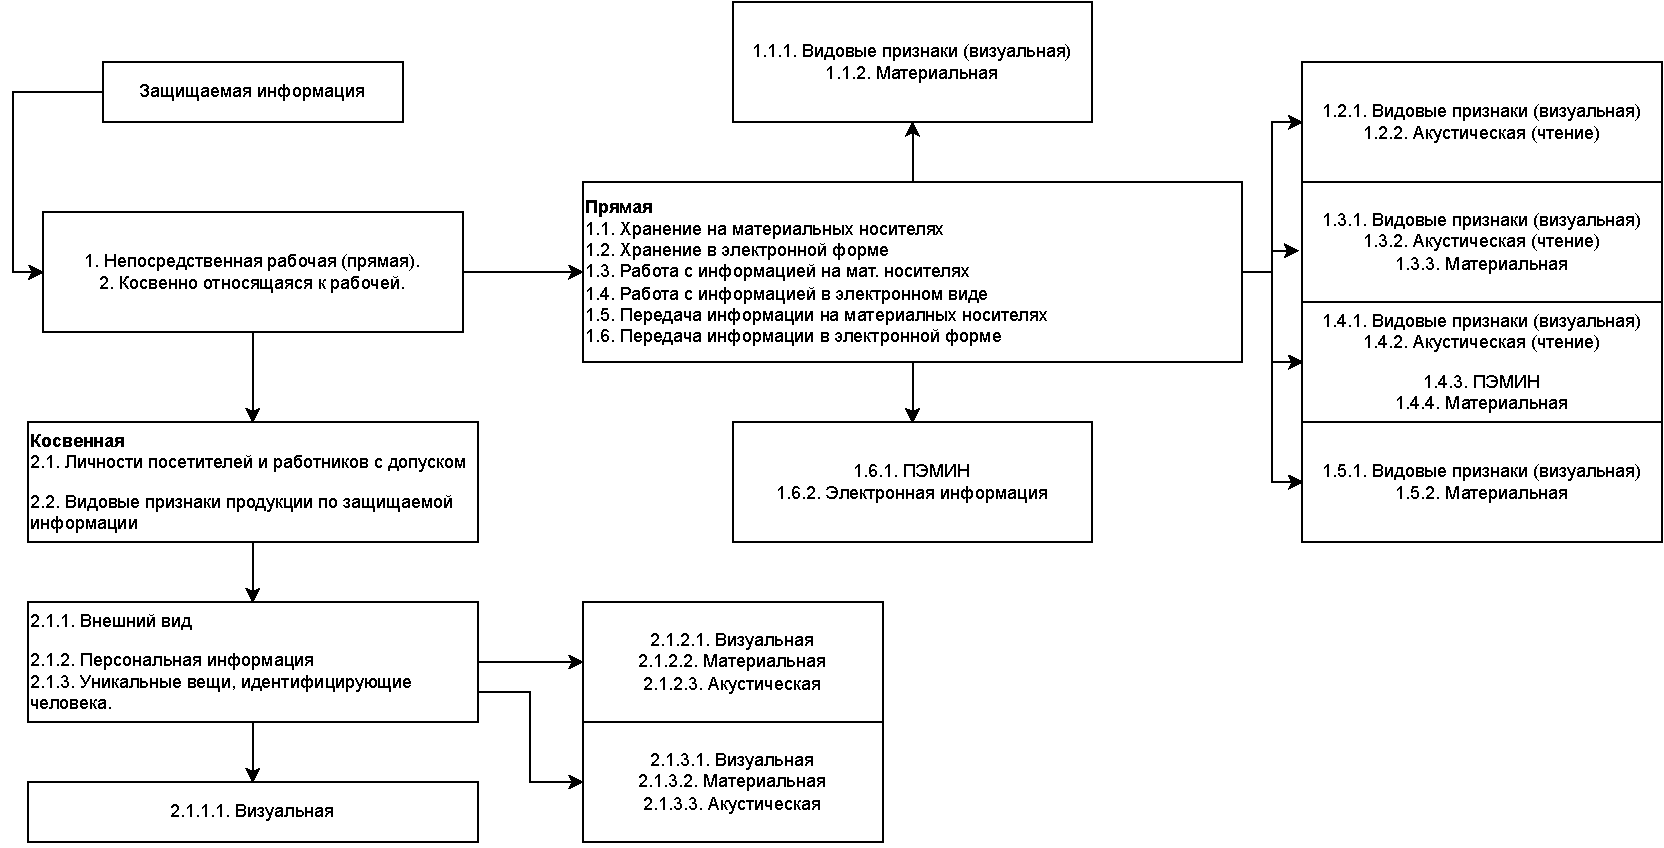
\includegraphics[scale=0.6, angle=-90]{block}\\
  Рис. 1: Графическая иллюстрация типов защищаемой информации на разных уровнях.\\
\end{center}

\newpage
\section{Схемы защищаемого объекта}
\begin{center}
  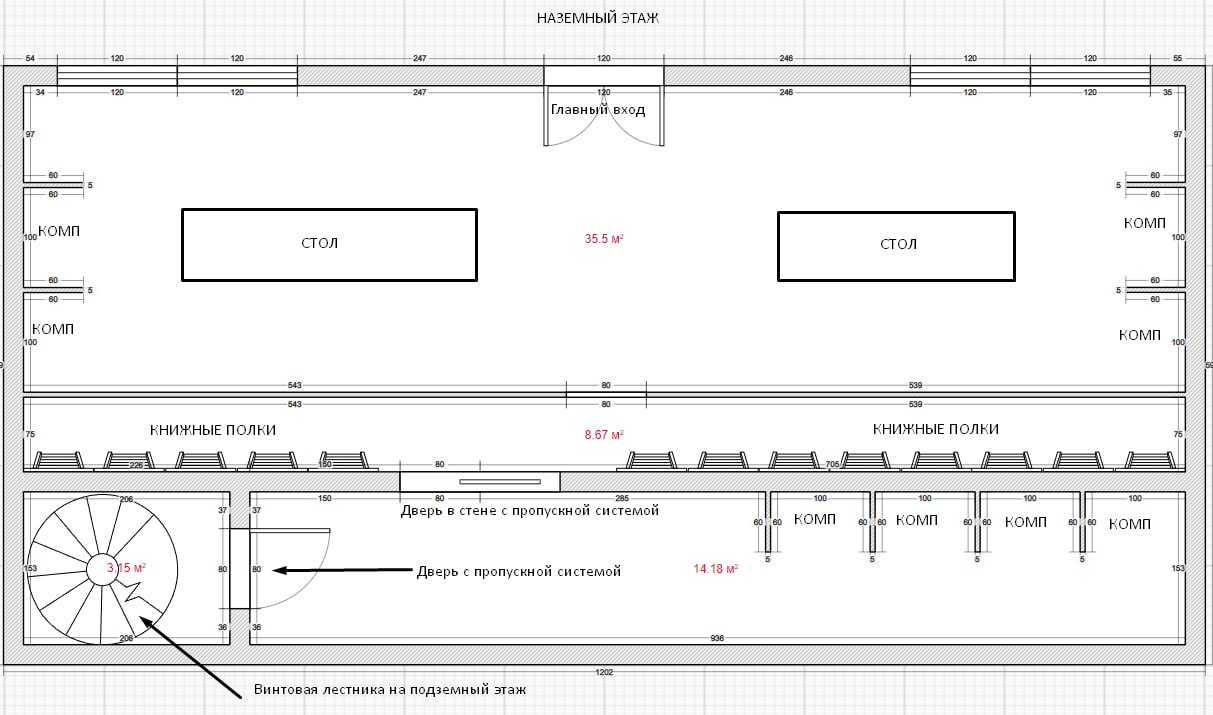
\includegraphics[scale=0.7, angle=-90]{shem1}\\

  Рис. 2: Графическая иллюстрация первого этажа здания.\\
\end{center}

\begin{center}
  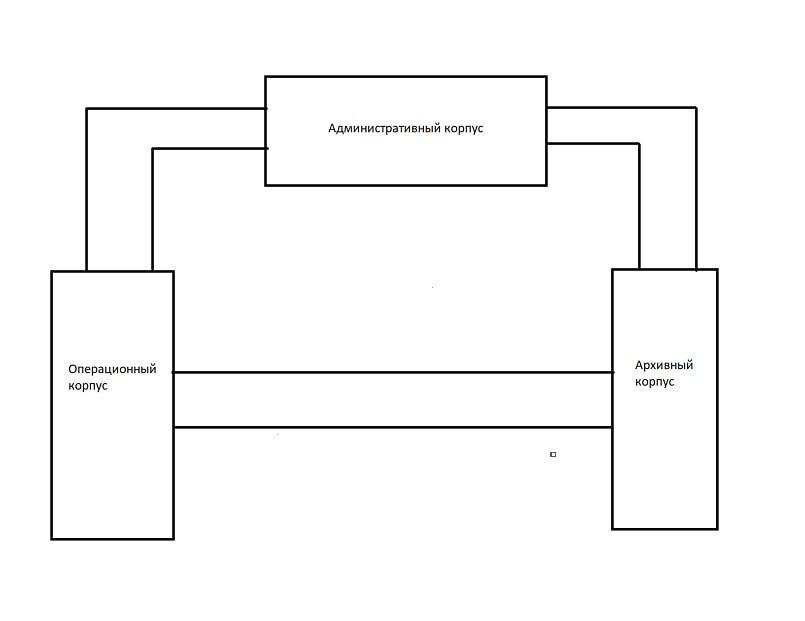
\includegraphics[scale=0.75]{shem2}\\

  Рис. 3: Графическая иллюстрация расположение корпусов и подземных переходов.\\
\end{center}

1.1. Работа с документами допуска "б" осуществляется в специально оборудованных
помещениях с видеонаблюдением и контрольно-пропускной системой.

1.2. На входе в каждое помещение осуществляется полный досмотр лицами,
которые отвечают за охрану помещений и имеют допуск уровня «б» или выше.

1.3. Помещения располагаются в подвальной части здания\\
(не имеют окон) и оборудованы шумоизоляцией и устройствами шумогенерации.

1.4. Для работы с информацией допуска «б» в разных корпусах здания
оборудованы специальные закрытые подземные переходы с собственной отдельной вентиляцией.


\begin{center}
  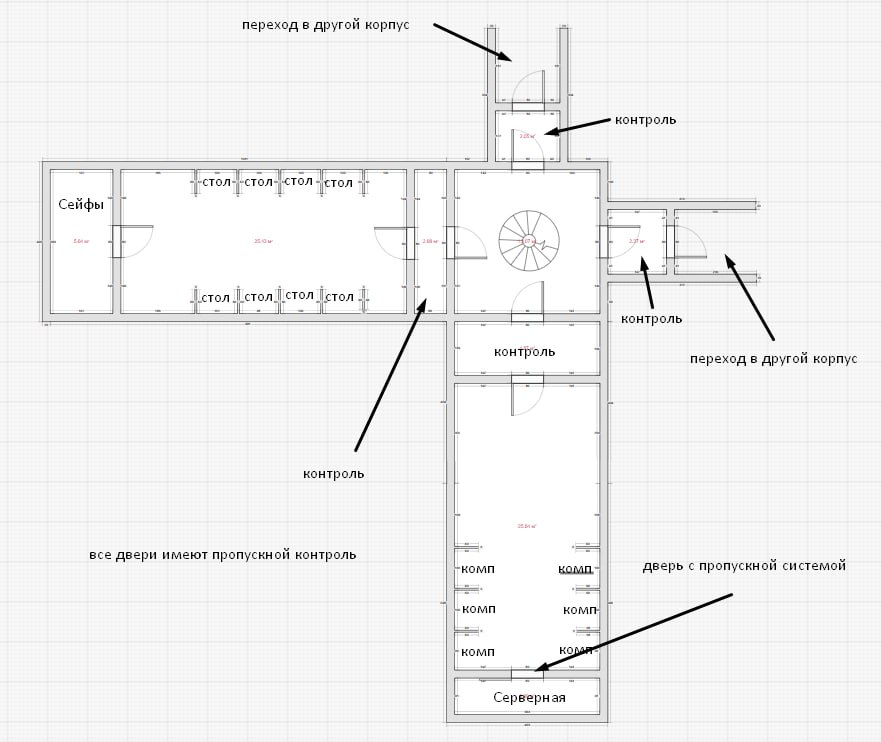
\includegraphics[scale=0.7]{shem3}\\

  Рис. 4: Графическая иллюстрация подвального помещения.\\
\end{center}

2.1. В каждом корпусе рядом со спец помещениями оборудованы специальные
закрытые серверные комнаты, в которых хранится информация с камер
видеонаблюдения в спец помещениях, электронные копии документов
допуска «a» и сведения о перемещениях всех сотрудников и посетителей.

2.2. Подвальные спец помещения оборудованы дренажной системой с насосом,
имеющей отдельные водоотводы обособленно от канализации в целях безопасности.

2.3. Материалы со спец допуском «б» хранятся в закрытом помещении в бумажном
виде. Работа с ними производится строго в этом помещении.

2.4. Каждый пакет документов хранится в отдельной бумажной непрозрачной папке.

2.5. Документы распределены по металлическим ячейкам, оборудованным
электронными замками.

2.6. После работы с документами необходимо вернуть их на исходное место
(в отведенные ячейки)

2.7. При отключении электричества - все электронные замки на ячейках
внутри и на входной двери - закрываются без возможности открыть до
включения питания.

2.8. Специально оборудованные помещения имеют отдельную закрытую
вентиляционную систему.

\subsubsection{ПЭМИН}

3.1. Экранирование помещения. Помещение должно быть защищено от
электромагнитных излучений с помощью специальных материалов, таких
как фольга или металлическая сетка. Это позволит снизить уровень
электромагнитных наводок и помешает получить доступ к данным.

3.2. Защита кабелей и сетей. Кабели и сети должны быть защищены от
электромагнитных наводок с помощью экранирования и использования
специальных фильтров. Это позволит снизить вероятность утечки
данных через ПЭМИН.

% 3.3.Использование защищенных систем хранения данных. Данные \\
% должны храниться на защищенных серверах, которые обеспечивают высокий 
% уровень безопасности и защиты данных от злоумышленников.

% 3.4.Ограничение доступа к системам и данным. Доступ к системам 
% и данным должен быть ограничен только для авторизованных пользователей 
% с помощью сичных паролей и аутентификации.

% 3.5.Регулярное обновление систем безопасности. Системы безопасности 
% должны регулярно обновляться и проверяться на наличие уязвимостей, 
% чтобы предотвратить возможные атаки.


\subsubsection{Хранение и использование документов в электронной форме.}

4.1.1. В электронном виде хранятся исключительно материалы со спец
допуском «а».

4.1.2. Хранение электронной формы на закрытом сервере.

4.1.3. Доступ к информации происходит только со специально
оборудованных ПЭВМ администрации и главных инженеров путем включения
в локальную сеть без доступа в интернет.

4.1.4. ПЭВМ оборудованы таким образом, что невозможно подключить/снять
какие-либо информационные накопители. Пользователь может только
читать информацию через защищенное приложение.

4.1.5. Данные о каждом входе в приложение сохраняются на защищенном сервере.

4.1.6. Помещения Администрации, главных инженеров корпусов и
главы секции информатизации в которых устанавливаются ПЭВМ оборудованы
на входе электрическим замком, открыть который можно только персональными
ключ-картами. Замки надежно закрываются автоматически при закрытии двери.

4.1.7. Администрация, главные инженеры корпусов и глава секции
информатизации имеют допуск «б» и оснащенные места с ПЭВМ для работы
с документами допуска «а».


\subsubsection{Хранение и использование документов допуска "a" в бумажном виде.}

4.2.1. Все бумажные версии материалов со спец.допуском «а» должны
храниться в запираемых шкафах или сейфах.

4.2.2. Доступ к документам осуществляется в специально отведенные
дни и часы.


\section{Личности работников с допуском. Персональная информация.}

5.1. Помещения оборудованы системой электронных пропусков. Каждый
пропуск представляет из себя личную карту с данными её владельца и
уровнем допуска.

5.2.Для доступа в личный кабинет (в случае работников и администрации)
и доступа к документам допуска уровня «б» необходим электронный пропуск.

5.3. На закрытый сервер поступают данные о перемещении и взаимодействии
с конкретными ячейками всех пользователей электронных пропусков.

5.4. В случае утраты пропуска одного из сотрудников/посетителей,
он сразу блокируется и выпускается новый.

5.5. Запрещено проносить в спец помещение любые носители информации.

5.6. Косвенная информация, касающаяся личных данных работников, уровень их
допуска, подробной статистики их посещений и передвижений внутри корпусов,
хранится в отдельных каталогах на защищенном сервере.

5.7. Персонал, имеющий допуск и работающий в закрытых секторах, не имеет
какой-либо специальной формы и других отличительных особенностей.

5.8. Доступ к информации по посетителям библиотеки с формами допуска $"$а$"$ и $"$б$"$ имеют работники библиотеки с допусками формы
$"$а$"$ и $"$б$"$ соответствено, притом персонал с допуском по форме $"$б$"$ может работать с посетителями с допуском по форме $"$а$"$
и без допуска вовсе, так же как $"$а$"$ может работать с простыми посетителями.

5.9. Информация по посетителям библиотеки с формами допуска хранится (а также обрабатывается и читается) на тех же ПЭВМ, что и информация
по остальным пользователям, но для доступа требуется персональная ключ-карта сотрудника с определённой формой допуска, описанной в п. 5.8.

\newpage
\subsubsection{Защита косвенной информации помимо персонала.}

5.1.1.Отсутствие прямых вывесок с указанием закрытых секций.

5.1.2.С пользователями защищаемых документов обсуждение происходит
внутри защищённого помещения.

5.1.3. Двери в закрытые секции закрыты электонными замками, оборудованы
доводчиками.

\end{document}